\documentclass{article}
\setlength{\parskip}{0pt} % esp. entre parrafos
\setlength{\parindent}{3pt} % esp. al inicio de un parrafo
\usepackage{amsmath} % mates
\usepackage{listings}
\usepackage[sort&compress,numbers]{natbib} % referencias
\usepackage{url} % que las URLs se vean lindos
\usepackage[top=15mm,left=20mm,right=20mm,bottom=25mm]{geometry} % \textbf{\textbf{}}margenes
\usepackage{hyperref} % ligas de URLs
\usepackage{graphicx} % poner figuras
\usepackage{subfigure}
\usepackage[spanish]{babel} % otros idiomas
\hypersetup{
    colorlinks=true,
    linkcolor=blue,
    filecolor=blue,      
    urlcolor=blue,
    citecolor=black,
}

\title{TAREA \# 12 \\ Red neuronal} %titulo
\author{Natalia Berenice P\'{e}rez L\'{o}pez} % author
\date{\today}

\begin{document} % inicia contenido

\maketitle % cabecera

\section{Objetivo}
El objetivo de esta práctica es estudiar de manera sistemática el desempeño de la red neuronal en términos de su puntaje F (F-score en inglés) para los diez dígitos en función de las tres probabilidades asignadas a la generación de los dígitos (ngb), variando a las tres en un experimento factorial adecuado.

\section{Desarrollo} % seccion y etiqueta
Para generar el código de esta práctica se realizaron algunas ideas y pruebas iniciales, las cuales se encuentran en \href{https://github.com/nataliaperez0/Simulation/tree/main/Tarea12}{mi repositorio}  en GitHub. Se inició tomando como base el código para la red neuronal de los digitos \citep{1} revisado en clase. Las modificaciones que se le realizaron al código fueron: establecer tres vectores de tres niveles cada uno con las probabilidades de cada color $negro$, $gris$ y $blanco$, agregar tres ciclos \texttt{for} para variar dichas probabilidades y otro para hacer $12$ réplicas de cada combinación $ngb$, también se agregó el código para obtener el puntaje $F$ o $F-score$ y un \texttt{data.frame} para almacenar la combinación $ngb$, el número de réplica y el $F-score$ correspondiente.
\smallskip

A continuación se muestra el fragmeto modificado en el código: 

\definecolor{verde}{rgb}{0,0.56,0.22}
\definecolor{codegray}{rgb}{0.5,0.5,0.5}
\definecolor{codegreen}{rgb}{0,0.56,0.22}
\definecolor{backcolour}{rgb}{0.95,0.95,0.92}
\definecolor{azul}{rgb}{0,0,1}

\lstdefinestyle{mystyle}{
    backgroundcolor=\color{backcolour},   
    commentstyle=\color{verde},
    keywordstyle=\color{azul},
    numberstyle=\tiny\color{codegray},
    stringstyle=\color{codegreen},
    basicstyle=\ttfamily\footnotesize,
    breakatwhitespace=false,         
    breaklines=true,                 
    captionpos=b,                    
    keepspaces=true,                 
    numbers=left,                    
    numbersep=5pt,                  
    showspaces=false,                
    showstringspaces=false,
    showtabs=false,                  
    tabsize=2
}

\lstset{style=mystyle}
\begin{lstlisting}[language=R, caption= Fragmento del código modificado.]
df = data.frame()
probn = c(0.98,0.65,0.35) #probabilidades negro
probg = c(0.95,0.75,0.55) #probabilidades gris
probb = c(0.45,0.10,0.005) #probabilidades blanco

for (ne in probn){
  for (g in probg){
    for (b in probb){
      for (replica in 1:12){
        modelos <- read.csv("digits.txt", sep=" ", header=FALSE, stringsAsFactors=F)
        modelos[modelos=='n'] <- ne
        modelos[modelos=='g'] <- g
        modelos[modelos=='b'] <- b
        
        r <- 5
        c <- 3
        dim <- r * c
\end{lstlisting}

Para el cálculo del $F-score$ se revisó la documentación sugerida por la Dra. Schaeffer \citep{2}, en la cual indica que la fórmula para obtener este puntaje es:  
\begin{equation}
\label{eq:e1}
F-score= 2\frac{precision * recall}{precision + recall} 
\end{equation}

En seguida se muestra el fragmento del código para obtener el puntaje $F$:

\lstset{style=mystyle}
\begin{lstlisting}[language=R, caption= Código para obtener el puntaje $F$.]
        print(contadores)
        #Calculo puntaje F-score
        precision = diag(contadores) / colSums(contadores[,1:10])
        recall = diag(contadores) / rowSums(contadores)
        fscore = (2 * precision * recall) / (precision + recall)
        result = c(ne, g, b, replica, fscore)
        df = rbind(df, result)
\end{lstlisting}

Utilizando el \texttt{data.frame} obtenido con el código anterior se realizó el diagrama caja-bigote combinado con diagramas de violín para analizar como varía el puntaje $F$ o $F-score$ con las diferentes combinaciones de probabilidades $ngb$ (Ver figura \ref{f1}). Con apoyo del repositorio de Navarro \citep{3} se cambiaron las etiquetas del eje $x$ en el diagrama.

\begin{figure} [h!]% figura
    \centering
    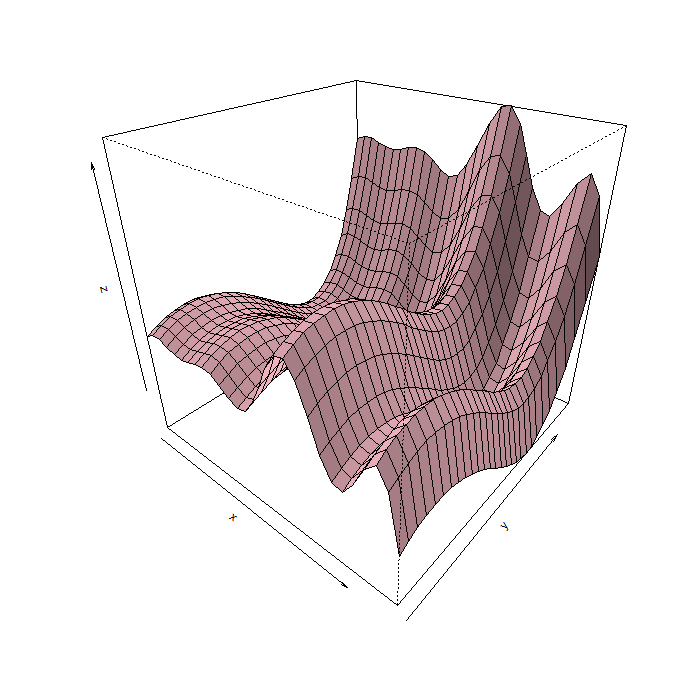
\includegraphics[width=15cm]{Figura1.png} % archivo
    \caption{Puntaje $F$ para cada combinación de probabilidades $ngb$.}
    \label{f1}
\end{figure}

En la figura \ref{f1} se puede observar que la combinación de probabilidades con la que se alcanza el mayor puntaje $F$ es la que presenta el máximo valor para negro y gris y el mínimo para blanco. Para analizar si existe una relación entre las combinaciones $ngb$ y el puntaje $F$ obtenido se realizó una prueba estadística. Se eligió realizar la prueba estadística \texttt{Kruskal Wallis} debido a que los datos no presentan normalidad.
\bigskip

En el cuadro \ref{Cuadro1} se  resumen los resultados de la revisión de los supuestos para poder aplicar la prueba estadística. El supuesto outliers se refiere a la cantidad de valores atípicos que existen en los grupos, la normalidad por grupos se obtuvo con la prueba de \texttt{Shapiro Wilk} y la homogeneidad de varianza se obtuvo con la prueba de \texttt{Levene}.

\begin{table}[ht]
\centering
\caption{Resultados del los supuestos para aplicar la prueba estadística.}
\smallskip

\begin{tabular}{ |p{2.1cm}|p{5cm}|}
 \hline
 Outliers & $47$ \\
 \hline
 Normalidad por grupo & $0.35/0.55/0.005$: $p$ = $1.72\times 10^{-6}$ $0.35/0.55/0.10$: $p$ = $1.81\times 10^{-4}$ $0.35/0.55/0.45$: $p$ = $1.06\times 10^{-4}$ $0.35/0.75/0.005$: $p$ = $1.62\times 10^{-7}$ $0.35/0.75/0.10$: $p$ = $2.05\times 10^{-6}$ $0.35/0.75/0.45$: $p$ = $2.43\times 10^{-4}$ $0.35/0.95/0.005$: $p$ = $2.35\times 10^{-6}$ $0.35/0.95/0.10$: $p$ = $4.48\times 10^{-6}$ $0.35/0.95/0.45$: $p$ = $2.02\times 10^{-4}$ $0.65/0.55/0.005$: $p$ = $5.30\times 10^{-5}$ $0.65/0.55/0.10$: $p$ = $2.37\times 10^{-2}$ $0.65/0.55/0.45$: $p$ = $2.31\times 10^{-2}$ $0.65/0.75/0.005$: $p$ = $3.42\times 10^{-3}$ $0.65/0.75/0.10$: $p$ = $3.93\times 10^{-4}$ $0.65/0.75/0.45$: $p$ = $1.16\times 10^{-5}$ $0.65/0.95/0.005$: $p$ = $6.09\times 10^{-3}$ $0.65/0.95/0.10$: $p$ = $8.46\times 10^{-4}$ $0.65/0.95/0.45$: $p$ = $7.73\times 10^{-5}$ $0.98/0.55/0.005$: $p$ = $6.68\times 10^{-4}$ $0.98/0.55/0.10$: $p$ = $2.58\times 10^{-1}$ $0.98/0.55/0.45$: $p$ = $4.47\times 10^{-4}$ $0.98/0.75/0.005$: $p$ = $8.90\times 10^{-6}$ $0.98/0.75/0.10$: $p$ = $1.25\times 10^{-1}$ $0.98/0.75/0.45$: $p$ = $3.07\times 10^{-3}$ $0.98/0.95/0.005$: $p$ = $8.79\times 10^{-15}$ $0.98/0.95/0.10$: $p$ = $2.38\times 10^{-6}$ $0.98/0.95/0.45$: $p$ = $1.34\times 10^{-3}$\\
 \hline
 Homogeneidad de varianza & $p$ = $3.43\times 10^{-22}$ \\
 \hline
\end{tabular}
\label{Cuadro1}
\end{table}

\bigskip
En los resultados se observa que para la normalidad en la mayoría de las combinaciones $p$ es menor a $0.05$, por lo tanto no se tiene normalidad.
\bigskip

Al realizar la prueba \texttt{Kruskal Wallis} se obtienen los resultados mostrados en el cuadro \ref{Cuadro2}.

\begin{table}[h!]
\centering
\caption{Resultados al aplicar la prueba estadística \texttt{Kruskal Wallis}.}
\smallskip

\begin{tabular}{ |p{2.1cm}|p{2.1cm}|}
 \hline
 Chi cuadrada & Valor de $p$ \\
 \hline
 $1603.7$ & $2.2\times 10^{-16}$ \\
 \hline
\end{tabular}
\label{Cuadro2}
\end{table}

Hipótesis nula : Las medias son iguales en todos los grupos.
\smallskip

Hipótesis alternativa: Debido a que $p < 0.05$ se rechaza la hipótesis nula, es decir que si existen diferencias significativas entre las medias de los grupos. 
\bigskip

Se entiende entonces que la variación de las probabilidades $ngb$ si tiene un efecto significativo en el puntaje $F$ de cada combinación.
\bigskip

A continuación se muestra el código utilizado para realizar la figura \ref{f1} y la prueba estadística \texttt{Kruskal Wallis}:

\lstset{style=mystyle}
\begin{lstlisting}[language=R, caption= Código para graficar y realizar la prueba estadística \texttt{Kruskal Wallis}.]
library(ggplot2)
library(tidyr)

etiq=rep(c("0.98,0.95,0.45","0.98,0.95,0.10","0.98,0.95,0.005","0.98,0.75,0.45","0.98,0.75,0.10","0.98,0.75,0.005","0.98,0.55,0.45","0.98,0.55,0.10","0.98,0.55,0.005",
              "0.65,0.95,0.45","0.65,0.95,0.10","0.65,0.95,0.005","0.65,0.75,0.45","0.65,0.75,0.10","0.65,0.75,0.005","0.65,0.55,0.45","0.65,0.55,0.10","0.65,0.55,0.005",
              "0.35,0.95,0.45","0.35,0.95,0.10","0.35,0.95,0.005","0.35,0.75,0.45","0.35,0.75,0.10","0.35,0.75,0.005","0.35,0.55,0.45","0.35,0.55,0.10","0.35,0.55,0.005"),
            times=c(12,12,12,12,12,12,12,12,12,12,12,12,12,12,12,12,12,12,12,12,12,12,12,12,12,12,12))
df$Etiquetas <- etiq 

library(reshape2)
df1 <- melt(df,id.vars='Etiquetas', measure.vars=c('0','1','2','3','4','5','6','7','8','9'))

png("Figura1.png", width=15, height=15, units="cm", res=1200)
gr = ggplot(df1, aes(x= Etiquetas, y= value))+ geom_violin(fill="pink", color="purple", lwd=0.2)
gr + geom_boxplot(width=0.4, fill="cyan", color="black", lwd=0.2, outlier.size = 0.6)+ labs(x="Combinacion de probabilidades (n,g,b)", y= "F-score") +
  theme(axis.text.x = element_text(angle = 90, vjust = 0.5, hjust=1))
graphics.off()

library(tidyverse)
library(ggpubr)
library(car)
library(rstatix)
library(rapportools)
library(readr)
library(gridExtra)

#PRUEBA ESTADISTICA...
#Estadisticas descriptivas
df1 %>%
  group_by(Etiquetas) %>%
  get_summary_stats(value, type = "mean_sd")

#SUPUESTOS PARA ANOVA
#1:Outliers
df1 %>%
  group_by(Etiquetas) %>%
  identify_outliers(value)

#2:Normalidad por Shapiro
tapply(df1$value, df1$Etiquetas, shapiro.test)

#3:Homogeneidad de varianza con prueba Levene
df1 %>%
  levene_test(value~Etiquetas)

#PRUEBA ESTADISTICA KRUSKAL WALLIS
kruskal.test(value ~ Etiquetas, data = df1)
\end{lstlisting}

\section{Reto 1}
Como un primer reto, extiende y entrena la red neuronal para que reconozca además por lo menos doce símbolos ASCII adicionales, aumentando la resolución de las imágenes a $5$ x $7$ de lo original de $3$ x $5$  (modificando las plantillas de los dígitos acorde a este cambio).
\bigskip

Para este reto se utilizó como base el código para la red neuronal de los digitos \citep{1} y el código para la generación de imágenes aleatorias de dígitos \citep{4}, ambos revisados en clase. Se generó un nuevo archivo de texto \texttt{.txt} llamado $digits2$ el cual se encuentra en \href{https://github.com/nataliaperez0/Simulation/tree/main/Tarea12}{mi repositorio}, en este archivo se usan las iniciales de los colores para indicar cuál pixel es cuál yendo por renglones.
\bigskip

A continuación se muestra el fragmeto modificado en el código para el reto $1$: 

\lstset{style=mystyle}
\begin{lstlisting}[language=R, caption= Fragmento del código modificado para el reto $1$.]
modelos <- read.csv("digits2.txt", sep=" ", header=FALSE, stringsAsFactors=F)
modelos[modelos=='n'] <- 0.995
modelos[modelos=='g'] <- 0.92
modelos[modelos=='b'] <- 0.002

r <- 7
c <- 5
dim <- r * c

tasa <- 0.15
tranqui <- 0.99

tope <- 21
digitos <- 0:tope
k <- length(digitos)
contadores <- matrix(rep(0, k*(k+1)), nrow=k, ncol=(k+1))
rownames(contadores) <- 0:tope
colnames(contadores) <- c(0:tope, NA)
\end{lstlisting}

\definecolor{verde}{rgb}{0,0.56,0.22}
\definecolor{codegray}{rgb}{0.5,0.5,0.5}
\definecolor{codegreen}{rgb}{0,0.56,0.22}
\definecolor{backcolour}{rgb}{0.95,0.80,0.92}
\definecolor{azul}{rgb}{0,0,1}

\lstdefinestyle{mystyle}{
    backgroundcolor=\color{backcolour},   
    commentstyle=\color{verde},
    keywordstyle=\color{azul},
    numberstyle=\tiny\color{codegray},
    stringstyle=\color{codegreen},
    basicstyle=\ttfamily\footnotesize,
    breakatwhitespace=false,         
    breaklines=false,                 
    captionpos=b,                    
    keepspaces=true,                 
    numbers=false,                    
    numbersep=5pt,                  
    showspaces=false,                
    showstringspaces=false,
    showtabs=false,                  
    tabsize=2
}

\lstset{style=mystyle}
\begin{lstlisting}[language=R, caption= Matriz de confusión.]
   0  1  2 3 4  5  6 7 8 9 10 11 12 13 14 15 16 17 18 19 20 21 <NA>
0  3 11  0 0 0  0  0 0 0 0  0  0  0  0  0  0  0  0  0  0  0  0    0
1  0 11  0 0 0  0  0 0 0 0  0  0  0  0  0  0  0  0  0  0  0  0    0
2  0  0 12 0 0  0  0 0 0 0  0  0  0  0  0  0  0  0  0  0  0  0    0
3  3  0  7 1 0  0  1 1 0 0  0  0  0  0  0  1  0  0  0  0  0  0    0
4  0  0  0 0 0  1  0 0 0 0  0  0  7  2  0  0  0  0  0  0  0  0    0
5  0  0  0 0 0  0  0 2 0 0  0  0  1  1  1 11  0  0  0  0  0  0    2
6  7  0  1 0 0  0  1 0 2 0  0  0  0  0  0  0  0  0  0  0  0  0    0
7  0  0  1 0 0  0 11 0 0 0  0  0  0  0  0  0  0  0  0  0  0  0    0
8  7  2  0 0 0  0  0 0 0 0  0  0  0  0  0  0  0  0  0  0  0  0    0
9  0  2  0 0 0 15  0 0 0 0  0  0  1  1  0  0  0  0  0  0  0  0    0
10 0  0  1 0 0  0  0 0 2 0 11  0  0  0  0  0  0  0  0  0  0  0    1
11 0  0  0 0 0  0  0 0 0 0  0  0  0  0  0  0  0  0  3  0  0  0   10
12 0  0  0 0 0  0  0 0 0 0  0  0 15  0  0  0  0  0  0  0  0  0    2
13 0  0  0 0 0  1  0 0 0 0  0  0  0  6  0  0  0  0  0  0  0  1    1
14 0  0  0 0 0  0  0 0 1 0  1  0  0  0 17  2  0  0  0  0  0  0    0
15 0  0  0 0 0  0  0 0 3 0  0  0  0  0  0  7  0  0  0  0  2  0    1
16 2  0  0 0 0  0  0 0 0 0  0  0  0  0  0  0  3  7  0  0  1  3    0
17 3 11  0 0 0  0  0 0 1 1  0  0  0  0  0  0  1  0  0  0  0  0    4
18 0  0  0 0 0  0  0 0 0 0  0  0  0  0  0  0  0  0 12  0  0  0    0
19 0  0  0 0 0  0  0 0 0 0  0  0  0  0  0  0  0  0  0 13  0  0    0
20 0  0  0 0 0  0  0 0 0 0  0  0  0  0  0  0  0  0  0  0  0  0    9
21 0  8  0 0 0  0  0 0 0 1  0  0  0  0  0  0  0  1  0  0  0  0    1
\end{lstlisting}

\begin{figure} [h!]% figura
    \centering
    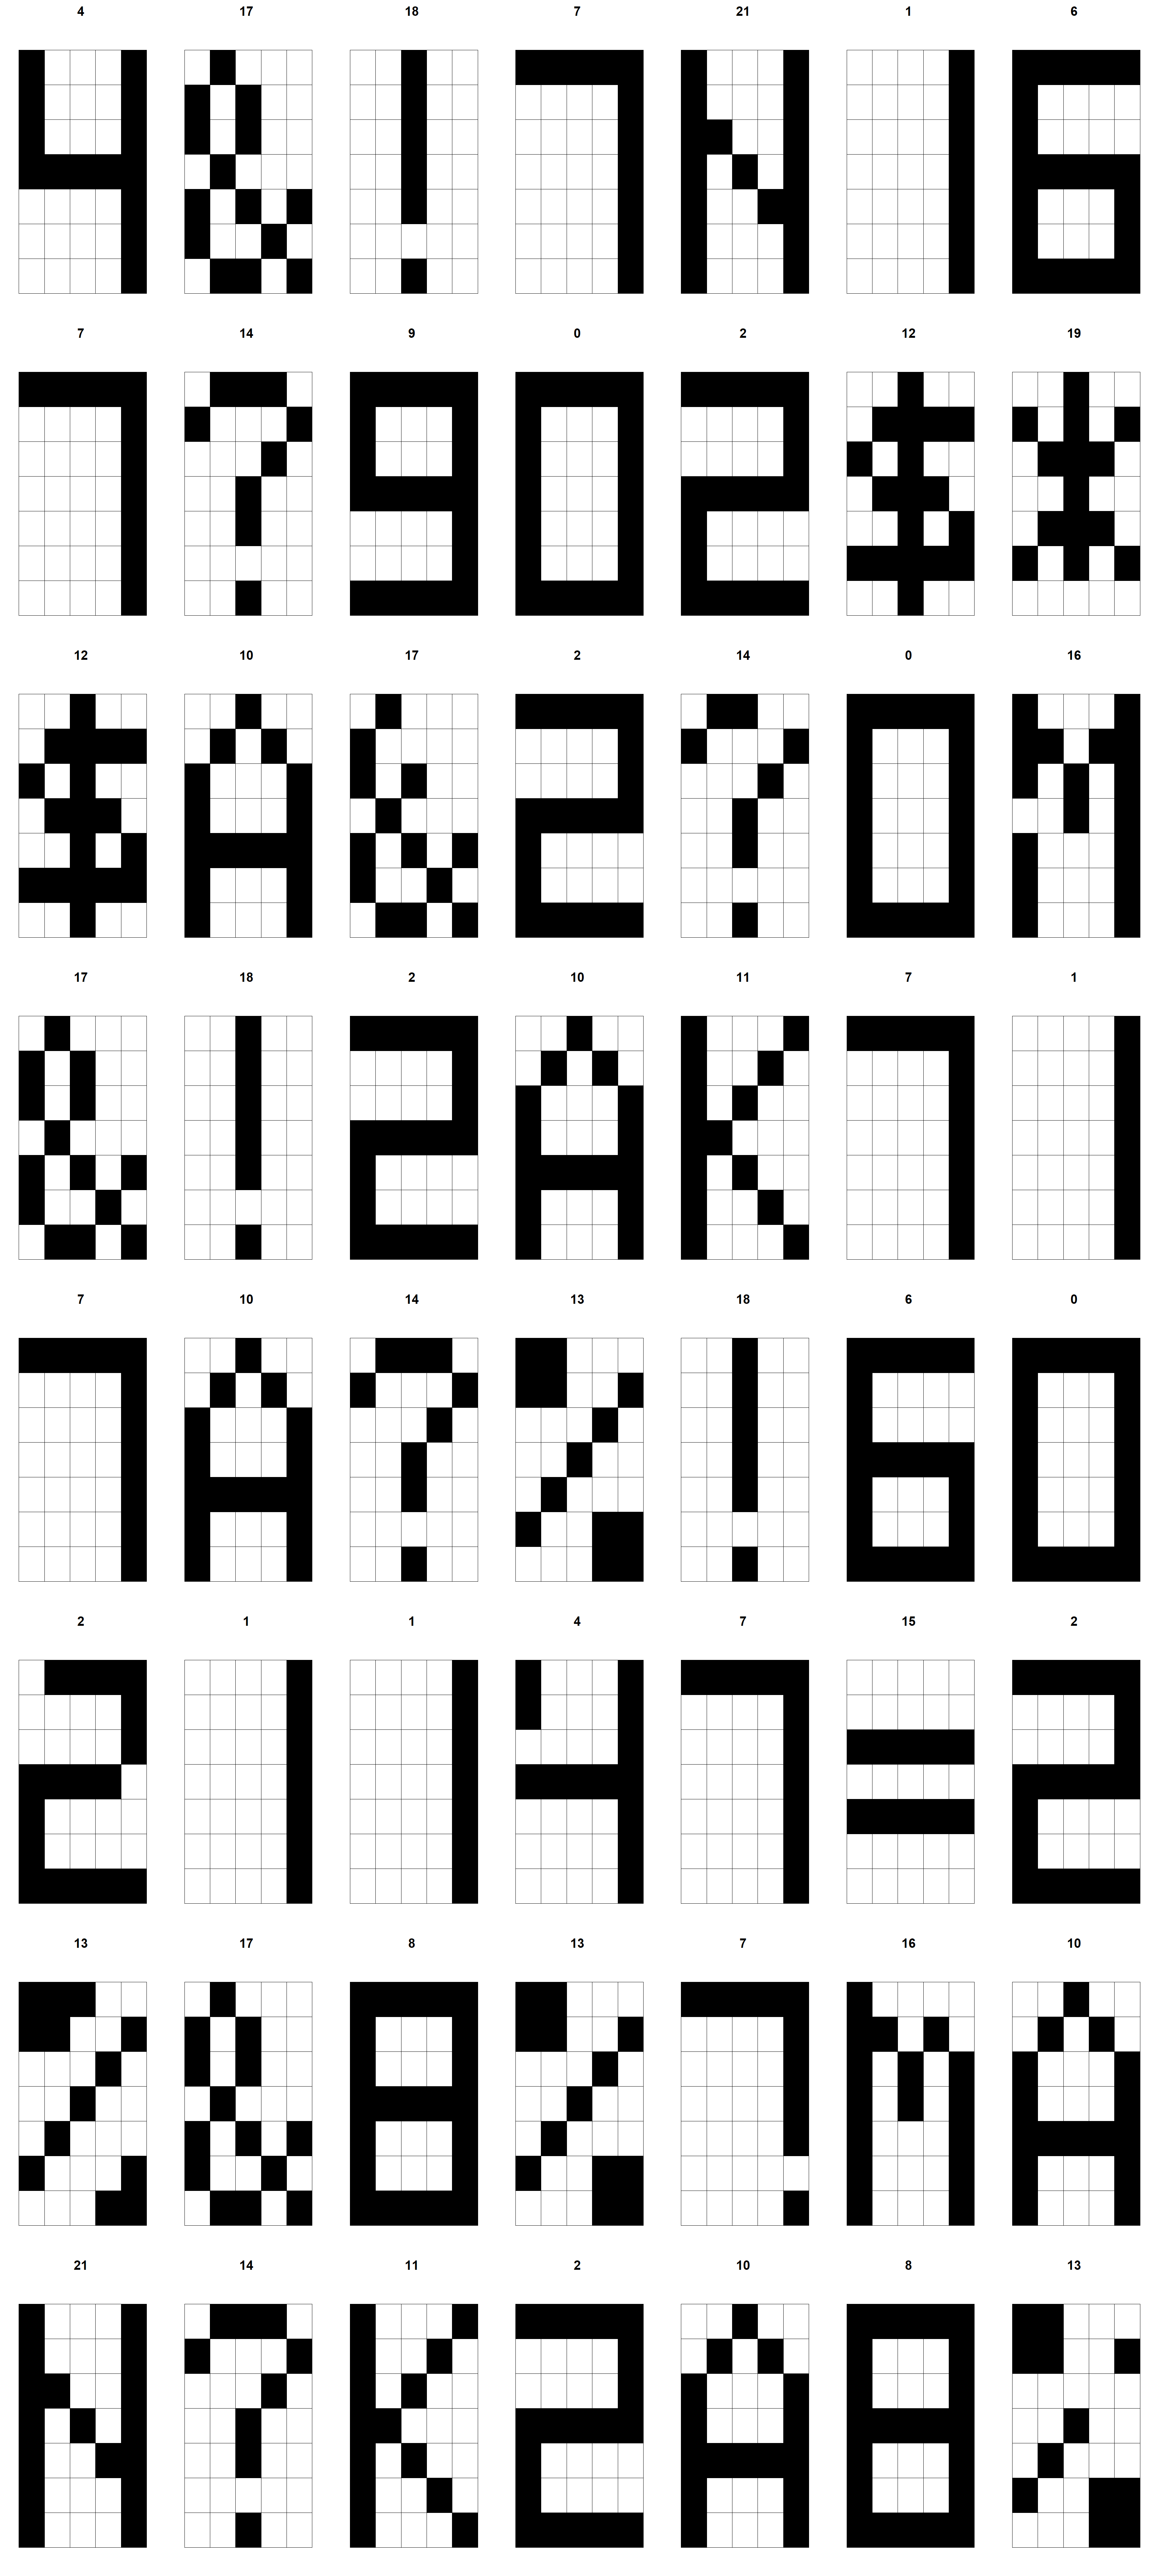
\includegraphics[height=9cm]{Figura2.png} % archivo
    \caption{Símbolos ASCII.}
    \label{f2}
\end{figure}

\newpage
\section{Conclusi\'{o}n}
Con base en el diagrama caja-bigote combinado con los diagramas de violín y el resultado de la prueba estadística, puedo concluir que el puntaje $F$ o $F-score$ aumenta dependiendo de la combinación de las probabilidades $ngb$, en la figura \ref{f1} se observa que la mejor combinación es $n$ = $0.98$, $g$ = $0.95$ y $b$ = $0.005$, es decir un alto valor para negro y un muy bajo valor de blanco ya que de esta manera se disminuyen las probabilidades de errores al identificar los números, también se puede ver que al disminuir los valores de $n$ y aumentar los valores de $b$ se obtiene un menor puntaje $F$ debido a que aumenta la posibilidad de no identificar correctamente los números. 
\smallskip

\newpage

\bibliography{referencias}
\bibliographystyle{plainnat}

\end{document}